%\documentclass[11pt]{amsart}
\documentclass[a4paper]{article}

\usepackage[colorlinks=true]{hyperref}
\usepackage{graphicx}
\usepackage{float}
%\usepackage{listings}
\usepackage{natbib}
\usepackage[usenames, dvipsnames]{color}

\title{Planning Document for ScalABM}
%\author{David R. Pugh, Daniel F. Tang, J. Doyne Farmer}
\date{\today}

\begin{document}
\maketitle

\section{Objective}

ScalABM is a \textit{community driven}, \textit{open-source} project to develop a \textit{user-friendly} modeling platform and tool stack for building \textit{scalable}, \textit{data-driven}, and \textit{reproducible} agent-based models (ABMs) of \textit{economic} systems on the JVM using \href{http://www.scala-lang.org/}{Scala} and \href{http://akka.io/}{Akka}. The purpose of this document is to provide both an introduction to ScalABM and to coordinate, prioritize, and plan future work on the project. 

\section{Motivation}

Failure to predict changes to economic systems is costly. According to the Dallas Federal Reserve Bank~\citep{Luttrell2013Costs} the recent financial crisis cost the United States on the order of 15 trillion dollars, suggesting a much larger cost for the world as a whole. These costs were significantly
born by the poor, who suffered directly from the downturn in housing markets, which caused many to default.

A variety of techniques have attempted to improve the prediction of economic behaviour. Dynamic Stochastic General Equilibrium (DSGE) models have made significant progress in assessing the underlying forces guiding macro-level behaviour~\citep{Smets2003,Sungbae2007BaysianDSGE}. However, DSGE models are somewhat limited, in that they are constructed under the presumption that human behaviour is homogeneous and that economic systems move toward an equilibrium~\citep{Farmer2009NeedABM}. This rests in stark contrast to the heterogeneous, analytically intractable human behaviour which underlies large-scale economic systems.

Agent-based models (ABMs) attempt to overcome these obstacles. ABMs allow heterogenous agent behaviour, permitting the researcher to consider the effects of complex micro-level interactions on macro-level behaviour. ABMs have had several successes~\citep{Klimek2015144,Poledna2014199,Deissenberg2008541,Schelling1971}. However, whilst ABMs offer heterogeneous behaviour for free, much of the research currently conducted is of a qualitative nature. Further, progress in the building of large scale models of economic systems has been significantly hindered by the lack of a common modelling platform as well as a common tool stack for data management and analytics. The consequence is that, even when ABM offer quantitative results, it is difficult to replicate or compare competing models.

\section{Solution: ScalABM}

ScalABM attempts to solve several of the problems in predicting and analysing the behaviour of economic systems. ScalABM merges the quantitative analysis of DSGE models with the heterogeneity and inherent scalability of ABMs. Further ScalABM offers replicable analysis by presenting a common, modular platform for using ABMs to scrutinizing a variety of economic systems. 

The intention of ScalABM is to provide a collaborative application where users in a variety of economic disciplines can model and analyse agent-based models. To the user the system will be accessed through a web-application, permitting the user to a.) import data, b.) set up their economic components using ScalABMs plug and play markets and institutions, and c.) analyse the dynamics of their model over time.
\\
\\
\textbf{ScalABM is}:

\begin{itemize}

\item \textit{Data Driven:} ScalABM we will manage the flow and storage of both model generated data as well as real-world data. The user's models will be grounded by their empirical data. Calibration and validation techniques will permit the user to adjust their model to fall in line with historical data whilst analytic tools will provide the user data on the state of the model during run-time.

\item\textit{Versatile:} With multiple entry points, ScalABM offers users their choice in the granularity of control required for their research. At the simplistic end, a user may instantiate plug-and-play markets, banks, and individuals via a web interface. Analysis of agent interactions can be conducted without any programming on the end-user side. If the user requires more granular control of their system, they may implement their own types of markets, banks, etc. By developing classes which meet the ScalABM's specifications, a user can develop the system to their own specification.

\item \textit{Open-Source:} The development of all ScalABM libraries will be driven by the needs of the economics ABM community. All software development will take place in public: from the start of the project all source code for the ScalABM project will be hosted on GitHub under a permissive Apache 2.0 license that allows for free use of the software libraries (even in commercial applications).

\item \textit{Modular:} ScalABM libraries are structured in a way that minimizes the amount of development time needed to reconfigure and existing model or build a completely new model. In order to maximize reuse of code, models built using our toolkit should be composed of mostly existing components. Leveraging mostly existing components reduces development time for a new model.

\item \textit{Scalable:} System size is a key parameter for modeling economic systems and in order to accurately model the dynamics of some systems, users may need to build and simulate models that are as close to observed scale as possible. ScalABM outsources cluster management to third party providers. ABMs built using our framework can be ``containerized'' using technologies such as \href{https://www.docker.com/}{Docker} or \href{https://www.vagrantup.com/}{Vagrant} and then deployed on a third-party cloud computing service provider such as \href{http://aws.amazon.com/}{AWS}, \href{https://cloud.google.com/compute/}{Google Compute Engine}, \href{https://www.heroku.com/}{Heroku}, \href{https://mesosphere.com/}{Mesosphere}, etc. This third party provider then handles all of the intricacies involved with scaling up the model on the cluster to meet our needs.
    
\item \textit{Reproducible:} No longer dependent on access to university or national supercomputers enhances the reproducibility or our research.  The ability to ``containerize'' an ABM built using ScalABM's framework means that researchers not directly involved in developing a model can still access everything (even down to the operating system) necessary to completely reproduce that model's output. The container can be used to run the model locally on a laptop or sent to a third party provider to scale up via the cloud.

\end{itemize}

\section{Deliverables}

Such a large project requires the coordination of many moving parts. This document makes a preliminary attempt at diagnosing all the high-level tasks in the hopes of planning and prioritizing them. This project can be broken down into several high-level tasks, broadly classified under ``Tools for Analysing Economic Systems" and ``Software Architecture and Quality Infrastructure". 
\\
\\
\textbf{Tools for Analysing Economic Systems:}
\\
\\
Tasks under this classification represent the agent-based economic system and the tools and components used to manipulate the economic system. These tasks represent the components the user will need to access whilst conducting research.

\begin{itemize}
	\item \textbf{Economic System Interface}: What are the requirements (i.e. interfaces) for markets, contracts, and individual agents? What are the possible actions for each type of agent? 
    \item \textbf{Agent Behaviour}: How does an individual agent learn, process information, and act?
    \item \textbf{Communication Layer}: How do the above systems interact and communicate? 
    \item \textbf{Calibration}: What tools are needed to calibrate a model to historical data?
    \item \textbf{Validation}: What tools are required to validate predictions? Can null-hypotheses be instantiated in a plug and play manner?
    \end{itemize}
\\
\\
\textbf{Software Architecture and Quality Infrastructure:}
\\
\\
These tasks represent the underlying infrastructure of ScalABM, as well as the controls put in place to maintain quality assurance. 

\begin{itemize}
	\item \textbf{High-level Software Architecture}: How is the UI separated from the model? What languages and databases are used?
    \item \textbf{Data processing}: How is data imported, processed, and accessed?
    \item \textbf{User Interface}: How will an end-user interact with the application? 
    \item \textbf{Open-Source Contributions}: How are open-source contributions managed and requested?
    \item \textbf{Website}: What is the best way to advertise ScalABM? How should open-source contributions be linked to the site?
    \item \textbf{Quality Management}: How are internal and open-source contributions reviewed and quality maintained?
    \end{itemize}

Below, each task is reviewed in turn. Particular focus is made toward enumerating the requirements and deliverables of each sub-task. This document will be extended as requirements are fleshed out. 

\section{Tools for Analysing Economic Systems}

\subsection{Economic Systems Interface}
\label{Interface}

The intention of ScalABM is to provide multiple and flexible entry points for analysing a variety of economic systems. To do this, the user must have flexibility in the creation of the components of their economic system. For example, the nuances of a market must be altered to meet each user's needs. However, where possible, ScalABM intends to permit generic, plug-and-play components for users who do not require additional complexity. 

To strike this balance, ScalABM offers an Interface for components of economic systems. These define the minimum requirements for each component. Once the APIs are finalized, ScalABM will offer simple concrete instantiations as plug and play components. Additional components will also be available via open-source contributions.

The interface for economic components consists in the following atomic components. The specifications of each of these components are currently in their design phase and will be extended shortly.

\begin{itemize}
	\item \textit{Actor}: Each \texttt{Actor} has a \texttt{Balance Sheet} and the ability to act on \texttt{Promises}. \texttt{Actors} are banks, corporations, and individuals. They are the atomic acting agent underlying ScalABM.
    \item \textit{Balance sheets}: A list of the assets and liabilities of each \texttt{Actor}. Assets and liabilities consist of \texttt{Goods} and \texttt{Promises}. 
    \item \textit{Goods}: \texttt{Goods} represent physical objects which possess some value.
    \item \textit{Promises}: A \texttt{Promise} represents a commitment between two (or more) \texttt{Actors} to undertake certain actions, potentially involving both \texttt{Goods} and additional \texttt{Promises}, specified by some \texttt{Sentence} when a certain \texttt{StateofAffairs} has occurred. For a more complete definition of the \texttt{Promise} API, please see Appendix~\ref{Promise API}. 
    \item \textit{Markets}: A \texttt{Market} provides some infrastructure for \texttt{Actors} to exchange \texttt{Goods} and \texttt{Promises}. The working low-level version of the \texttt{Market} API can be found in Appendix~\ref{Market API}.
    \item \textit{Sentences}: A \texttt{Sentence} is the logical language of promises. They not only define what assets to transfer, but also explain under what circumstances the trade will go forward. No API currently exists, but the preliminary thought is to use a contract language as described in \citet{Bahr2015certified}, \citet{bahr2014towards}, and \citet{Andersen2006}.
\end{itemize}

\subsubsection{Plug and Play Components}

Once the design of the interface has stabilized, ScalABM will generate a group of concrete instantiations of the interfaces which can be used as plug-and-play markets, promises, etc. A list, however, should be constructed prior to the design of the interfaces so that the developers can keep use-cases in mind when designing the interface. Additionally, open-source contributions of additional extensions to the interface will be made available online (see Section~\ref{opensource}) 

\subsection{Agent Behaviour}
\label{Agent Behaviour}

An economy is populated with a variety of agents (i.e., consumers, producers, financiers, government, etc). ScalABM's goal with the behavioral layer is to distill the core essence (in terms of data and behaviors) of these different agents into a multi-layered API defining a generic \textit{economic agent} that can then be specialized to the various types of economic agents needed for any particular model.

Several key features distinguish \textit{economic} agents from more generic types of agents. At a minimum these features include: purpose driven (or goal oriented) behaviour, an ability to learn, and the ability to anticipate future events. This suggests that our behavioral layer will need APIs for:
\begin{itemize}
    \item \textit{Goals or objectives (and their associated behavioral rules)}: Our goals and objectives API needs to be as un-opinionated as possible as prospective users of ScalABM are likely to have strong opinions on how to define appropriate goals and decision rules for their agents. At the same time, we will need to have some type of underlying null model of agent goals/objectives. Utility maximization, Belief-Desire-Intent (BDI), probabilistic discrete choice (AKA, random utility maximization) are possibilities.
    \item \textit{Learning rules}: A large number of various learning rules/mechanisms have been proposed in the academic literature. Roughly, learning rules seem to fall into two camps: learning through previous experience (e.g., reinforcement learning) and learning through observation (e.g., belief learning). Useful references for learning rules for ABMs are the two handbook chapters \href{http://web.uvic.ca/~mingkang/econ353/project/Brenner.pdf}{Brenner (2006)} and \href{http://www.socsci.uci.edu/~duffy/papers/duffy2006.pdf}{Duffy (2006)}.
    \item \textit{Expectations formation rules}: A large number of various expectation formation rules have been proposed in the literature. Useful references for expectation formation rules are \href{http://feb.kuleuven.be/fac/Slides_Degrauwe/HomHBchapter23.pdf}{Hommes (2006)}, \href{http://econ.columbia.edu/files/econ/content/hommes_background_material_2.pdf}{Anufriev and Hommes (2012)}, \href{http://www.columbia.edu/~mw2230/AREcon.pdf}{Woodford (2013)}, \href{http://www.emeraldinsight.com/doi/pdfplus/10.1108/S0193-230620140000017002}{Assenza et al (2014)}.
\end{itemize}

Figure~\ref{fig:BehaviorImage} depicts a high-level description of an agent as a layered collection of behaviors and decision rules.

\begin{figure*}
\centering
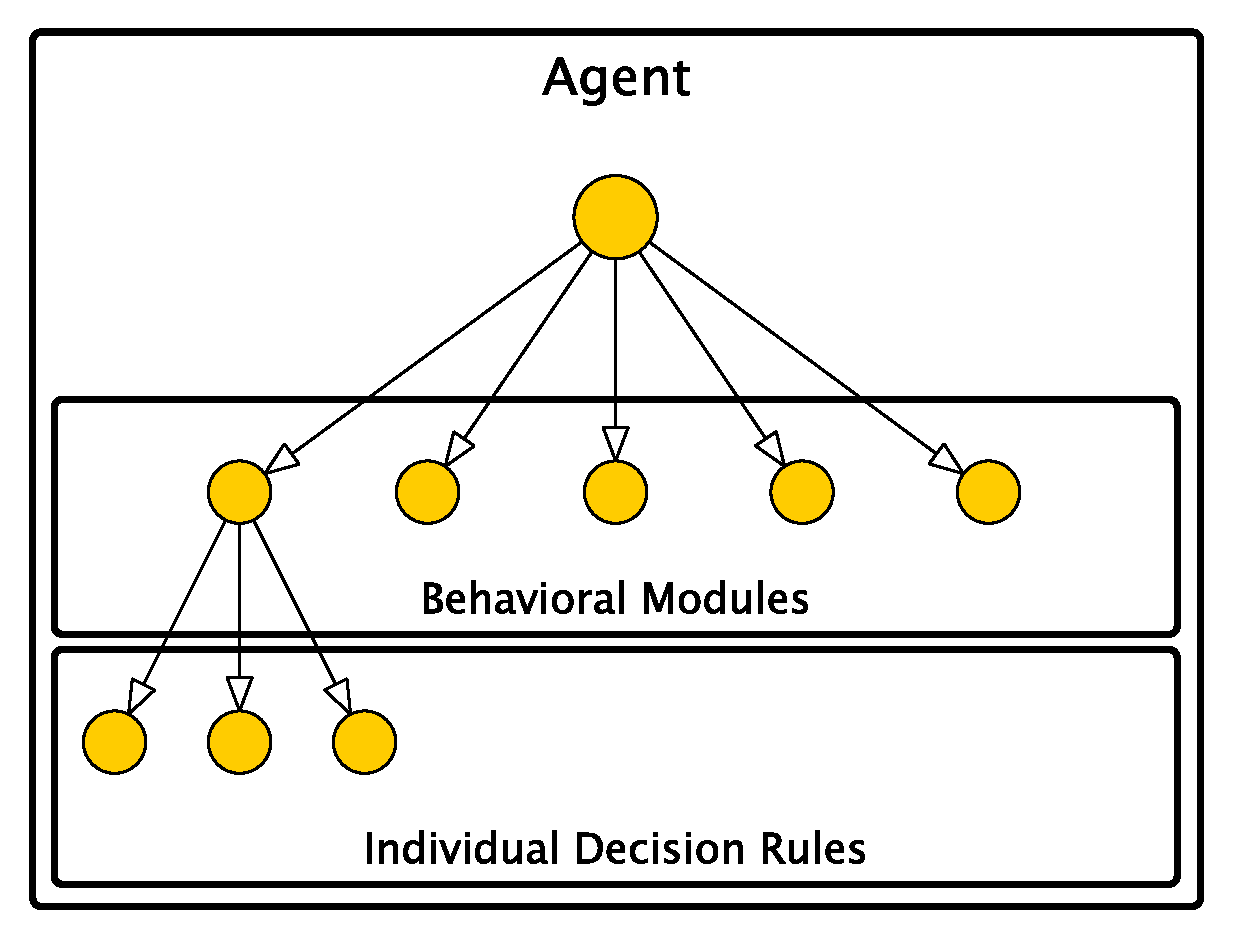
\includegraphics[width=10cm]{img/hierarchical-actor.pdf}
\caption{An agent in our framework is a layered collection of behaviors and decision rules.}
\label{fig:BehaviorImage}
\end{figure*}

Our economic agents will need to condition their decisions on an information set. In contrast to (most) DSGE models, information sets in our framework will be highly heterogeneous. The information set for any particular economic agent should consist of three components:
\begin{itemize}
    \item Private information: information that is idiosyncratic to a particular agent. 
    \item Public information: information that a particular agent shares with one or more agents.
    \item Global information: information that is shared between all agents.
\end{itemize}

\begin{figure}[H]
\centering
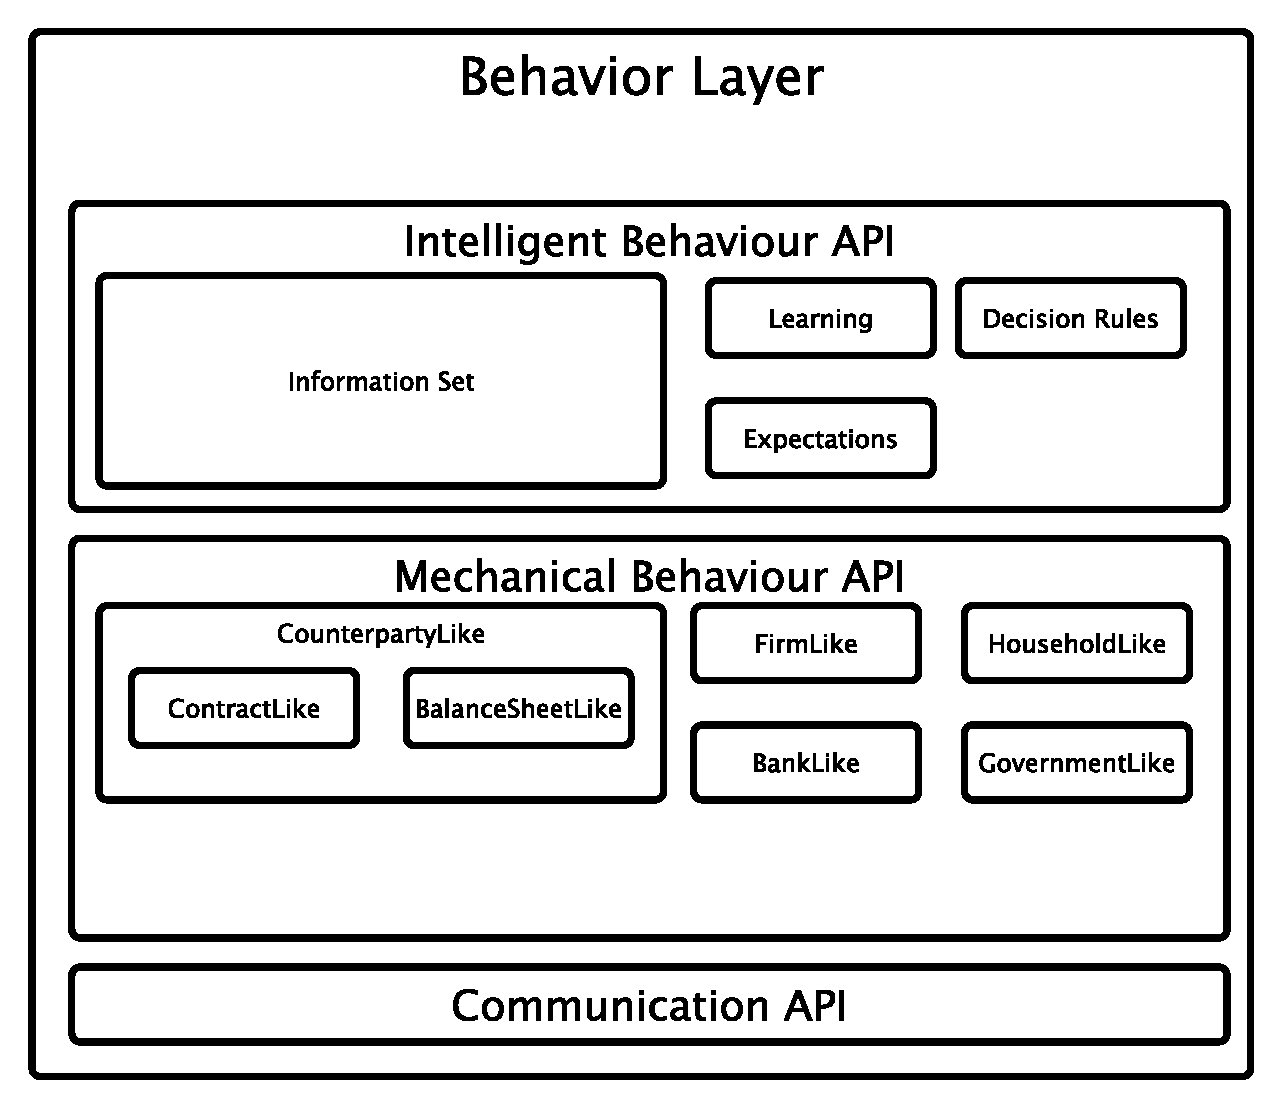
\includegraphics[width=10cm]{img/behavior-layer.pdf}
\caption{Behavioural layer: Incorporates all Actor behaviour with inter Actor communication.}
\label{fig:BehaviouralLayer}
\end{figure}

\subsection{Communication Layer}
\label{CommunicationLayer}

Sections~\ref{Interface} and~\ref{Agent Behaviour} define the components of an economic system, but not how these components interact. Concurrent communication between real-world economic agents is a fundamental fact of economic life. Inter-agent communication can be either direct (i.e., ``peer-to-peer'') or indirect (i.e., via market institutions). In order to model both direct and indirect communication between agents in our framework we leverage the \href{https://en.wikipedia.org/wiki/Actor_model}{Actor model} of concurrency. The Actor model treats ``actors'' as the universal primitives of concurrent computation: in response to a message that it receives, an actor can make local decisions (given its information set), send more messages, determine how to respond to the next message received, etc.

Figure~\ref{fig:BehaviouralLayer} illustrates how this communication layer resides in the behavioural layer. In order to impose structure on inter and intra agent communications we have developed an API for a scalable agent communication language for economic agents tentatively called ScalACL. The ScalACL API specifies:

\begin{itemize}
    \item a set of abstract message types that impose structure on the messages passed between a group of economic agents,
    \item a set of abstract protocols that impose structure on conversations (i.e., sequences of messages) between a group of economic agents,
    \item a behavioral trait that allows an agent to communicate using the language.
\end{itemize}
Each abstract message type can be thought of as defining an ``envelope'' containing the actual content of the message that is to be exchanged between a group of economic agents. Defining envelopes containing messages is useful because it allows agents to react based on the type message received. Each abstract protocol defines a particular subset of message types that can be sent by an agent in response to a particular type of message that it has received. Our agent communication API is influenced by, but not slave to, the \href{http://www.fipa.org/}{Foundation for Intelligent Physical Agents (FIPA)} compliant \href{http://www.fipa.org/specs/fipa00037/SC00037J.pdf}{Agent Communication Language (ACL)}.

Finally, the process of wiring model components together (which includes the specification of all model parameters, agent behavioral strategies, etc), sometimes called dependency injection (DI), should be as simple and transparent as possible. The wiring process should be specified in a single, \textit{human-readable}, model configuration file. The build process (i.e., specification of dependencies, platform specific build options, etc) for a particular model should be completely specified in a single build file.

\subsection{Calibration}
\label{Calibration}

If a user is attempting to understand an existing economic system, they will need to calibrate the interaction of their economic components such that the entire system mimics historical data. Example calibration questions include:

\begin{itemize}
    \item Historically, how do individuals process information to make decisions?
    \item How does the scarcity of resources affect market dynamics? 
	\item What variables (or non-linear combination of variables) provide the most predictive force when compared to historic data?
    \end{itemize}

The intention of the calibration tools is to allow 1.) linking dataset variables to model parameters, 2.) feature selection, and 3.) predictive analysis of how economic components interact.

\subsubsection{Associating historic variables to model parameters:}

At the simplest level, calibration involves syncing some variable in the imported, historic data with a variable in the model. For example, the temperature in a dataset may need to be linked to a temperature model parameter. ScalABM should provide some user-friendly mechanism for associating values in the dataset to parameters in the model. Though the most simple 1:1 example is given, thought should go into a user-friendly design for more complicated cases. As mentioned in Section~\ref{CommunicationLayer}, this will hopefully be accomplished via a configuration file --- though the details still need to be discussed.

\subsubsection{Feature Selection}

In an attempt to simplify their model, users may seek to diagnose the parameters which offer the most explanatory historic effect. Discussion needs to occur, regarding to what level ScalABM will offer tools to support this operation.
There are a variety of techniques available for feature selection, and often these solutions will simultaneously perform predictive analysis:

\begin{itemize}
    \item Genetic Algorithms
    \item Random Forests
    \item etc... 
\end{itemize}

Future discussion should prioritize algorithms which are better at uncovering non-linear interactions.

\subsubsection{Prediction Analysis}

Prior to attempting to uncover experimental effects, the model should be calibrated to historic data. If, at some starting point $t_0$, the model is able to predict the historic flow of the economic system, then there is a greater likelihood that the model can accurately predict the movement of the system in novel state space (i.e. the future). 

Again, discussion is required to define to what extent ScalABM will provide predictive analysis tools. Potential tools include, but are not limited to (for a nice comparison of several techniques, see~\citealp{Bajari2015machinelearning}):

\begin{itemize}
    \item Neural Networks
    \item Random Forests
    \item Linear Regression 
    \item Support Vector Machines
    \item Bagging
    \item Kalman Filters~\citep{Ward150703}
\end{itemize}

Further, research at INET is currently attempting to scaffold from calibration techniques in meteorology. Depending on the success of this project, such tools may be incorporated into ScalABM.

\subsection{Validation}
\label{Validation}

Validation tools will likely be integrated into the calibration tool set. However, conceptually it is worth discussing them separately. Validation tools work in coordination with calibration tools to: 

\begin{itemize}
    \item Generalize the predictive capacity of the model.
    \item Increase the likelihood that the model will accurately predict market behaviour in novel state space.
\end{itemize}

Validation aids in avoiding \href{http://en.wikipedia.org/wiki/Overfitting}{overfitting}, whereby the model is overly calibrated to historic data. Since most real-world behaviour involves a noisy process, perfectly mapping one's model to historic data attempts to capture the concept of noise as a predictive variable. This leads to poor predictions in novel state spaces. Validation techniques provide a mechanism for generalizing the predictive function, (hopefully) uncovering the more fundamental causative dynamics of the system. This will likely come in the form of \href{http://en.wikipedia.org/wiki/Cross-validation_(statistics)}{cross-validation}. By testing one's model on data the model have never consumed, the predictive capacity of the model in novel state spaces is increased.

As in the case of calibration techniques, future discussions should focus on whether ScalABM will integrate validation tools in their system.

\section{Software Architecture and \\ Quality Infrastructure}

\subsection{High-Level Software Architecture}

The high-level design of ScalABM's platform architecture should mimic the layered architecture of a \href{http://www.reactivemanifesto.org/}{reactive}, ``Fast Data'' web application. Figure \ref{fig:architecture} summarizes the high-level design of the platform architecture.\footnote{
See figure 1 from \href{./fast-data-big-data-evolved.pdf}{Wampler (2015)} for a similar high-level summary of a Reactive, ``Fast Data'' web application architecture.}

\begin{figure}
\centering
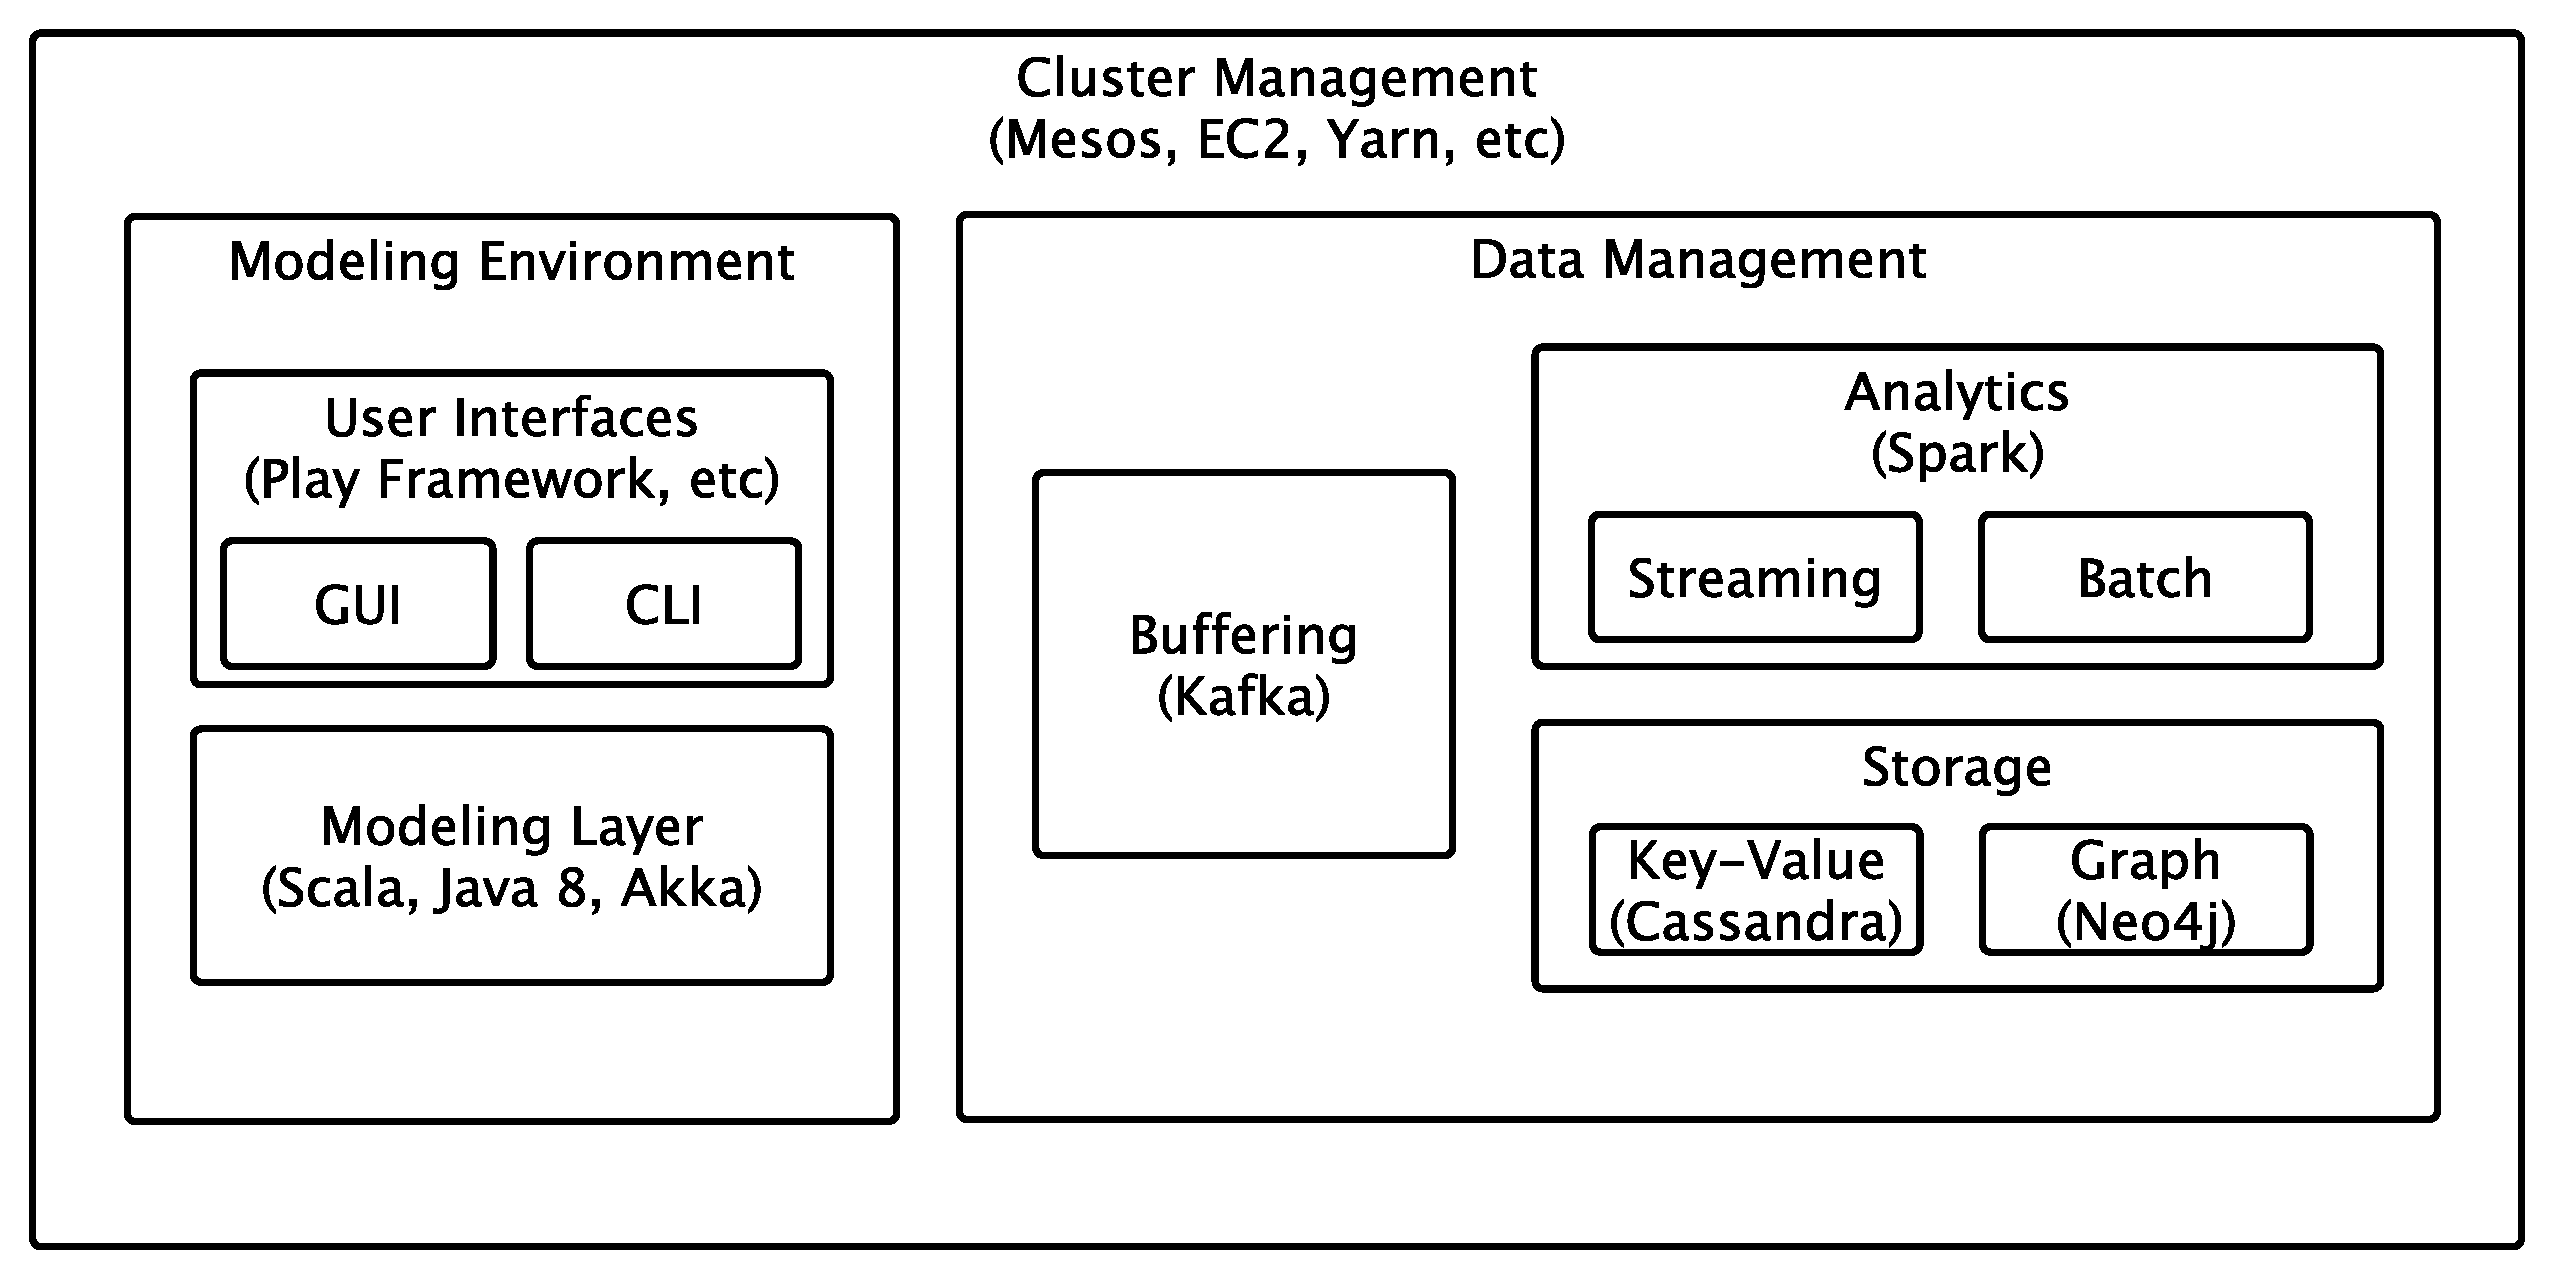
\includegraphics[width=12cm]{img/coarse-grain-schema-2.pdf}
\caption{High-level architecture design for ScalABM.}
\label{fig:architecture}
\end{figure}

\subsubsection{Cluster management} 
ScalABM attempts to provide increases in processing speed through parallelism and cluster management. Current approaches to running large-scale ABMs leverage either:
\begin{itemize}
    \item University/national super-computers: Use FLAME or Repast to build large-scale, complicated models. Both FLAME and Repast use some kind of message passing (but NOT ``peer-to-peer'' message passing) under the hood.
    \item GPU computing: Use CUDA, FLAME GPU (or similar) to build large-scale, simple models.
\end{itemize}
Our strategy for running ABMs at scale will instead leverage massively multi-core cloud computing clusters that are quickly becoming the dominant form of large-scale computing outside of academia. Benefits to this approach include:

\begin{itemize}
    \item Outsourcing of cluster management to third party providers. ABMs built using ScalABM can be ``containerized'' and sent off to a third-party cloud computing service provider such as \href{http://aws.amazon.com/}{AWS}, \href{https://cloud.google.com/compute/}{Google Compute Engine}, \href{https://www.heroku.com/}{Heroku}, \href{https://mesosphere.com/}{Mesosphere}, etc. This third party provider can then handle all of the intricacies involved with scaling up the model on the cluster to meet the users needs.
    \item No longer dependent on access to university/national super-computers enhances the reproducibility or our research.  The ability to ``containerize'' an ABM built using out framework means that researchers not directly involved in developing a model can still access all material necessary to completely reproduce that model's output. The container can be used to run the model locally on a laptop or sent to a third party provider to scale up via the cloud. 
\end{itemize}

\subsubsection{Modeling environment}
The modeling environment consists of user interfaces and the modeling layer. The ``back end'' of the modeling environment is the modeling layer which consists of the actual source code libraries used to implement our ABMs (see Sections~\ref{Interface} and~\ref{Agent Behaviour} for more detail). Important characteristics of the modeling layer are that:  

\begin{itemize}
    \item The modeling layer should facilitate the construction of new ABMs out of pre-existing, modular components. Novel model components should be able to easily extend pre-existing components. 
    \item Model configuration, including specification of all model parameters as well as the ``wiring'' of model components, should be specified in configuration files that are separate from the actual source code.
\end{itemize}

The modeling layer itself is organized into a number of sub-layers: a behavioral layer, an information layer, and a data analytics layer. See figure \ref{img-figure-2}.
\begin{figure}[H]\label{img-figure-2}
\centering
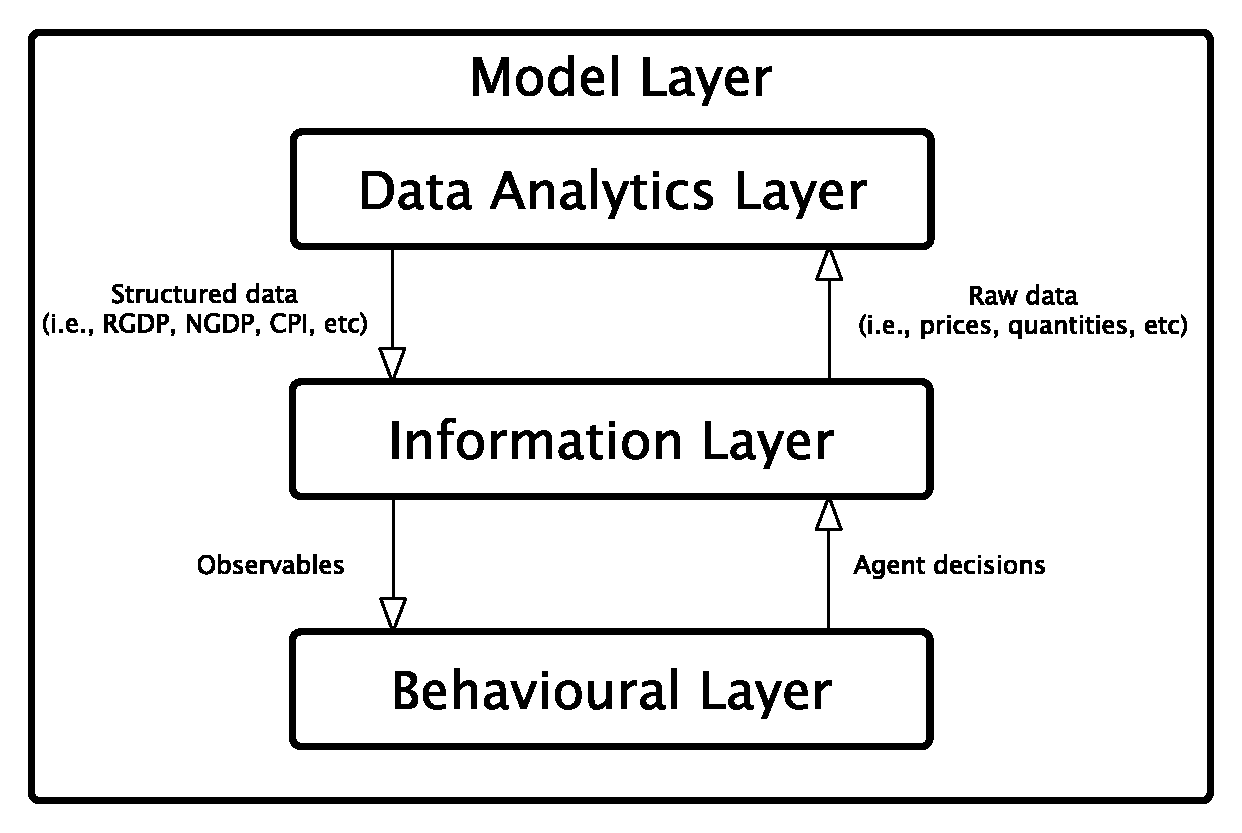
\includegraphics[width=10cm]{img/coarse-grain-model-layer.pdf}
\caption{High-level organization of the modeling layer.}
\end{figure}

\subsection{User Interface}

The ``front end'' of the modeling environment consists of two, complementary user interfaces.

\begin{enumerate}
    \item A user-friendly, web-browser based graphical user interface (GUI). The GUI should facilitate interactive exploration of an existing model in near real-time.  The GUI should support real-time data streaming, analysis, and visualization.
    \item An intuitive and consistent command line interface (CLI). In addition to facilitating efficient batch processing of model simulations (e.g., parameter sweeps), the CLI should allow for easy replication of any particular model simulation.
\end{enumerate}

The designs of both UIs require extensive discussion. Even before design discussions can occur, preliminary questions include: 

\begin{itemize}
     \item Who is the intended audience for the GUI and CLI? i.e. How simplistic must the UI be?
     \item What is the priority of the UI compared to the back-end modelling layer?
     \item Will the primary contributors of the UI be from INET or from the open source community?  
    \end{itemize}
  
  
\subsection{Data Processing}

In order for our ABMs to be data-driven, we need to think carefully about how our framework will manage the flow and storage of data (both model generated data as well as real-world data). There are (at least) three components to data management: access, analytics, and storage.
\begin{itemize}
    \item Access: A running ABM will generate a large volume of data. Model generated data might be stored, sent to a data analytics engine, or logged out to a file(s). Additionally, data will likely flow in the reverse direction.  In particular, agents in a running ABM may need to read data from a data store (for example, one might wish to initialize economic agents using real-world data).
    \item Analytics: A running ABM is a continuous source of data whose volume is not predetermined. Put another way, ABMs generate \href{http://www.reactive-streams.org/}{reactive data streams}.  The data analytics components should therefore include tools for processing and analyzing streaming data. In addition to processing and analyzing streaming data, there is also a need to preform various ``batch'' or ``mini-batch'' computations. Such batch processing jobs would be performed either relatively infrequently on streaming data or upon completion of a model simulation. The data analytics should include tooling for dealing with batch computations.
    \item Storage: The modeling layer should have read/write access to a scalable data store. Additionally, the data analytics components will need a source of input data. In order to avoid simulations being I/O bound, our data store should have extremely fast write access.
\end{itemize}

\subsubsection{Data Management}
Broadly speaking, we will need to store two types of data: real-world data and model generated data. The way in which we store our data should be heavily influenced by the types of questions we intend to ask of our data. 
There are two kinds of questions that we will want to ask of our model generated data:
\begin{enumerate}
    \item Questions about cross-sectional and time series properties of model generated data. For these types of questions NoSQL Key-Value databases, such as \href{http://cassandra.apache.org/}{Cassandra},  are ideal data stores. Key-Value databases are designed for storing data in a schema-less way. In a key-value store, each datum consists of an indexed key and a value, hence the name. 
    \item Questions about the network structures between model agents. For questions about network structure, graph databases are ideal. Graph databases, such as Neo4j, are designed for data whose relations are well represented as a graph and has elements which are interconnected, with an undetermined number of relations between them.
\end{enumerate} 

\subsection{Website}

The website will act as the front-face of the application. As such its role will change as ScalABM advances. 

\subsubsection{First Phase}

At the planning stage of the product, the website will advertise ScalABM to potential:

\begin{itemize}
\item \textit{collaborators/investors}: The website should contain enough information to offer individuals a moderate understanding of the details of the project. Contact information should be available for deeper inquiries. Information should be presented with a bias toward potential collaboration.
\item \textit{open-source contributors}: Whilst the details of open-source contribution are being worked out, the website should advertise the intention of open-source contributions. If a potential contributor wishes to subscribe to a mailing list, this should be made available.
\end{itemize}

\subsubsection{Mid-Life}

During the mid-life of ScalABM the website will focus on:
 
\begin{itemize}
\item offering details and documentation of the product.
\item requesting open-source contributions.
\item where possible, offering prototypes for early adopters.
\item continuing to support collaborators/investors.
\end{itemize}

\subsubsection{Project Maturity}
When ScalABM is mature, the website will:
\begin{itemize}
\item advertise the use of the tool as an out-of-the-box solution for researching economic systems through ABMs.
\item describe how to use the product
\item offer online forums and discussions
\item continue to advertise how to contribute to extending the tool via open-source contributions.
\end{itemize}

\subsubsection{Planning}

From a planning perspective, the initial version of the website should be prioritized. Connecting with potential investors, collaborators, and contributors is vital for the long-term success of the project. Currently design is an open question which should be considered.

\subsection{Quality Management}

Quality control will need to consider internal management, as well as controlling external, open-source contributions.

\subsubsection{Internal Quality Management}
Development within INET will be quality controlled via a mixture of unit test cases, code reviews, and the encapsulation garnered from \href{https://www.atlassian.com/pt/git/workflows#!workflow-feature-branch}{feature branch workflow} and \href{https://help.github.com/articles/using-pull-requests}{pull requests}.

\begin{itemize}
  \item \textit{Unit Test Cases}: Code will be subject to \href{https://en.wikipedia.org/wiki/Unit_testing}{continuous unit testing}. Validation of test case code coverage will be automated (e.g. \href{https://coveralls.io/}{Coveralls}). Further, during code reviews, peers will validate that outlying use cases are considered within the test case suite.
  \item \textit{Code Reviews}: Part of a developer's responsibility is to review the code of their peers. These code review sessions will be scheduled at regular intervals and following \href{https://help.github.com/articles/using-pull-requests}{pull requests}.
  \item \textit{Feature Branch Workflow and Peer Requests}: In an attempt at encapsulation and decoupling, development will be compartmentalized into feature branches. Each feature of the application will be assigned a lead developer. This developer will act as a gatekeeper in maintaining the integrity and quality of that feature. Prior to integrating a feature into the main application (i.e. master branch), a pull request will be required. A peer review will take place prior to integration.
\end{itemize}

\subsubsection{Open Source Management}

The vetting and implementation of open-source contributions will play a significant part in quality management. This document discusses the planning of open-source contributions, including their quality management, as a whole in the next section. 

\subsection{Open-Source Contributions}
\label{opensource}
Several decisions must be made in order to manage the quality of open-source contributions. At a high-level, the contribution workflow needs to be defined. This flow will need to answer several open questions, including:

\begin{itemize}
\item How are potential contributors informed of ScalABM's needs? 
\item How are contributions vetted? 
\item When and how often will contributions be assimilated into a new build? 
\item Are different types of contributions vetted differently? For instance, if a contributor extends the Market interface to meet their own needs, does INET provide a repository where individuals can share their work with the community?
\end{itemize}

More fundamentally a discussion needs to address: 

\begin{itemize}
\item When should open source contributions be requested?
\item Are contributions going to be (at least initially) focused in a particular area of the project (e.g. the GUI)?
\end{itemize}

\section{Prioritization}

This section should contain the prioritization of the aforementioned tasks. What should happen when and what can happen in tandem? In the current, preliminary stage, perhaps the website and the design of the back-end Economic Systems Interface should be prioritized? A lot of the UI design will relate to how the back-end is implemented, and since the back-end design will invariably require some iteration, it may be a good idea to hold off on the front-end.

\section{Project Roles and Responsibilities}

This section will contain the points of contact for each of the high-level tasks once they are assigned. 

\section{Schedule}

This section will contain a schedule for the high-level tasks once it is made available. 

\appendix
\section{Promises API}
\label{Promise API}

\subsection{Definition of a \texttt{Promise}}
A \texttt{Promise} represents a commitment between a \texttt{promisor} and some \texttt{promisee} to undertake certain \texttt{actions}, potentially involving both \texttt{goods} and additional \texttt{promises}, specified by some \texttt{Sentence} \texttt{when} a certain \texttt{StateofAffairs} has occurred. 

These considerations lead to the following low-level interface for the \texttt{Promise} trait.

\begin{verbatim}
trait Promise {

  def promisor: ActorRef
 
  def promisee: ActorRef
  
  def actions: Sentence
  
  def when: StateOfAffairs

}
\end{verbatim}

Want to allow for the possibility that some promises can not be given (and therefore not transferred or exchanged) from one \texttt{Actor} to another \texttt{Actor}. To capture this feature we define a separate \texttt{GiveablePromise} trait.

\begin{verbatim}
trait GiveablePromise extends Promise {

  val isGiveable: Boolean

}
\end{verbatim}

\subsection{\texttt{Actions} over \texttt{Promises}}

\subsubsection{Uni-lateral \texttt{Actions}}
An \texttt{Actor} $i$ can \textit{unilaterally} decide to perform any of the following \texttt{Actions} with a \texttt{Promise}. 
\begin{itemize}
	\item \texttt{create} a new \texttt{Promise}: When an \texttt{Actor} creates a new \texttt{Promise}, the \texttt{Actor} becomes its \texttt{promisor} and the new \texttt{Promise} becomes a liability for that \texttt{Actor}. Similarly, the new \texttt{Promise} becomes an asset for which ever \texttt{Actor} is the \texttt{promisee}.
	\item \texttt{accept} a \texttt{Promise}: If an \texttt{Actor} $i$ chooses to \texttt{accept} a \texttt{Promise} from another \texttt{Actor} $j$, then the \texttt{Promise} is added as an asset to the balance sheet of \texttt{Actor} $i$ and as a liability to the balance sheet of \texttt{Actor} $j$.
	\item \texttt{reject} a \texttt{Promise}: An \texttt{Actor} $i$ can always choose to \texttt{reject} (i.e., \textit{not} \texttt{accept}) a \texttt{Promise} from another \texttt{Actor} $j$. Rejected promises are not added to balance sheets.
	\item \texttt{fulfill} a \texttt{Promise}: An \texttt{Actor} $i$ who is the \texttt{promisor} of a \texttt{Promise} may choose to perform \texttt{actions} specified in the \texttt{Sentence} \texttt{when} a certain \texttt{StateOfAffairs} has occurred. Once a \texttt{Promise} is successfully fulfilled, it is removed from both the balance sheet of its \texttt{promisor} and the balance sheet of its \texttt{promisee}.
	\item \texttt{break} a \texttt{Promise}: An \texttt{Actor} $i$ who is the \texttt{promisor} of a \texttt{Promise} may choose \textit{not} to perform \texttt{actions} specified in the \texttt{Sentence} \texttt{when} a certain \texttt{StateOfAffairs} has occurred. A decision to \texttt{break} a \texttt{Promise} is the same as a decision \textit{not} to \texttt{fulfill} a \texttt{Promise}.\footnote{
	%
	Breaking a \texttt{Promise} may or may not have consequences. Should consequences be specified in the original \texttt{Promise}? I think so.
	%
	} 
	\item \texttt{destroy} a \texttt{Promise}: An \texttt{Actor} $i$ who is the \texttt{promisee} of a \texttt{Promise} may choose to \texttt{destroy} that \texttt{Promise} prior to a certain \texttt{StateOfAffairs} occurring. Once destroyed a \texttt{Promise} is removed from both the balance sheet of the \texttt{promisee} \textit{and} the balance sheet of the \texttt{promisor}.   
	\item \texttt{give} a \texttt{Promise}: An \texttt{Actor} $i$ who is the \texttt{promisee} of a \texttt{Promise} may choose to \texttt{give} that \texttt{Promise} to another \texttt{Actor} $j$.
	\item \texttt{redeem} a \texttt{Promise}:  An \texttt{Actor} $i$ who is the \texttt{promisee} of a \texttt{Promise} may choose to \texttt{redeem} that \texttt{Promise} after a certain \texttt{StateOfAffairs} has occurred. Redemption of a \texttt{Promise} can be thought of as a request that the \texttt{promisor} of that \texttt{Promise} \texttt{fulfill} the \texttt{Promise}.
\end{itemize}

The above actions can be combined into a low-level, \texttt{PromiseMaker} trait that extends the \texttt{Actor} base trait:
\begin{verbatim}
trait PromiseMaker extends Actor {
  
  def create(promisee: ActorRef,
             actions: Sentence,
             when: StateOfAffairs): Promise
  
  def destroy(promise: Promise): Unit
  
  def accept(promise: Promise): Unit
  
  def reject(promise: Promise): Unit
  
  def fulfill(promise: Promise): Unit
  
  def break(promise: Promise): Unit
  
  def give(promise: Promise, other: ActorRef): Unit
  
  def redeem(promise: Promise): Unit
  
}
\end{verbatim}

\subsubsection{Cooperative \texttt{Actions}}
Two \texttt{Actors} $i$ and $j$ can cooperate \textit{bi-laterally} to perform additional actions over \texttt{Promises}:
\begin{itemize}
	\item \texttt{transfer} a \texttt{Promise}: An \texttt{Actor} $i$ who is the \texttt{promisee} of the \texttt{Promise} can \texttt{transfer} a \texttt{Promise} to \texttt{Actor} $j$ as follows:
	\begin{enumerate}
		\item \texttt{Actor} $i$ \texttt{give} \texttt{Promise} to \texttt{Actor} $j$
		\item \texttt{Actor} $j$ \texttt{accept} \texttt{Promise} from \texttt{Actor} $i$
	\end{enumerate}
	\item \texttt{exchange} of \texttt{Promises}: Two \texttt{Actors} $i$ and $j$ who are the \texttt{promisees} of different \texttt{Promises} can \texttt{exchange} these \texttt{Promises} with one another as follows:
	\begin{enumerate}
		\item \texttt{Actor} $j$ \texttt{create} new \texttt{Promise} \{\texttt{give} existing \texttt{Promise} to \texttt{Actor} $i$\}.
		\item \texttt{Actor} $j$ \texttt{transfer} new \texttt{Promise} to \texttt{Actor} $i$.
		\item \texttt{Actor} $i$ \texttt{transfer} existing \texttt{Promise} to \texttt{Actor} $j$
		\item \texttt{Actor} $j$ \texttt{fulfill} \texttt{Promise} to \texttt{Actor} $i$
	\end{enumerate}
\end{itemize}
A few things are worth noting about a bi-lateral \texttt{exchange}. First, by choosing to \texttt{fulfill} the new \texttt{Promise} in step 4, \texttt{Actor} $j$ gives his existing \texttt{Promise} to \texttt{Actor} $i$ (which completes the \texttt{exchange}). Second, the new \texttt{Promise} issued by \texttt{Actor} $j$ in step 1 involved a promise to \texttt{give} and \textit{not} a promise to \texttt{transfer} an existing  \texttt{Promise} to \texttt{Actor} $i$.\footnote{
%
Should it be possible to for an \texttt{Actor} to create a \texttt{Promise} that commits \textit{other} \texttt{Actors} to perform actions? Do we have any real world examples?.
%
}
Finally, note that an \texttt{exchange} could take place with \texttt{Actor} $i$ creating the new \texttt{Promise} in step 1. The important point is that either \texttt{Actor} $i$ or \texttt{Actor} $j$ (not necessarily both) must be able to \textit{credibly} commit to \texttt{give} its \texttt{Promise} upon receipt of the other's \texttt{Promise}.\footnote{
%
The credibility of any particular \texttt{Promise} should be endogenously determined within the model and \textit{not} imposed by us \textit{a priori}
%
}

It is interesting to compare the above bi-lateral exchange mechanism with a multi-lateral exchange mechanism involving cooperation between three \texttt{Actors} $i$, $j$, and $k$. Two \texttt{Actors} $i$, $j$ who are the \texttt{promisees} of different \texttt{Promises} can \texttt{exchange} these \texttt{Promises} using \texttt{Actor} $k$ as an intermediary as follows:
\begin{enumerate}
	\item \texttt{Actor} $k$ \texttt{create} new \texttt{Promise} \{\texttt{give} \texttt{Actor} $j$ \texttt{Promise} to \texttt{Actor} $i$\}.
	\item \texttt{Actor} $k$ \texttt{create} new \texttt{Promise} \{\texttt{give} \texttt{Actor} $i$ \texttt{Promise} to \texttt{Actor} $j$\}.
	\item \texttt{Actor} $k$ \texttt{transfer} new \texttt{Promise} to \texttt{Actor} $i$.
	\item \texttt{Actor} $k$ \texttt{transfer} new \texttt{Promise} to \texttt{Actor} $j$.
	\item \texttt{Actor} $i$ \texttt{transfer} existing \texttt{Promise} to \texttt{Actor} $k$
	\item \texttt{Actor} $j$ \texttt{transfer} existing \texttt{Promise} to \texttt{Actor} $k$
	\item \texttt{Actor} $k$ \texttt{fulfill} \texttt{Promise} to \texttt{Actor} $i$
	\item \texttt{Actor} $k$ \texttt{fulfill} \texttt{Promise} to \texttt{Actor} $j$
\end{enumerate}
An important feature of this multi-lateral process is that, so long as \texttt{Actor} $k$ can \textit{credibly} commit to \textit{both} \texttt{Actors} $i$ \textit{and} $j$, then the exchange between $i$ and $j$ can take place even if \textit{neither} \texttt{Actor} $i$ \textit{nor} \texttt{Actor} $j$ can bi-laterally commit to \texttt{give} its \texttt{Promise} upon receipt of the other's \texttt{Promise}.\footnote{
%
The difference between multi-lateral and bi-lateral commitment has been stressed by many monetary theorists, in particular Kiyotaki and Moore in a series of papers.
%
}
There are several interpretations of \texttt{Actor} $k$'s role in the above process.  One interpretation is that \texttt{Actor} $k$ is functioning as a central clearing party (CCP) for transactions between other \texttt{Actors}; another more institutional interpretation is that \texttt{Actor} $k$ is an actual \texttt{Market}.

One final cooperative action needs to be specified: \texttt{transfer} of a \texttt{Promise} that is liability for one \texttt{Actor} to some other \texttt{Actor}.  An \texttt{Actor} $i$ who is the \texttt{promisor} on a \texttt{Promise} can only \texttt{transfer} that \texttt{Promise} to another \texttt{Actor} $j$ with permission from the \texttt{promisee} of that \texttt{Promise}, \texttt{Actor} $k$. 
\begin{enumerate}
	\item \texttt{Actor} $i$ \texttt{create} new \texttt{Promise} \{\texttt{give} \texttt{Actor} $j$ existing \texttt{Promise} \}.
	\item \texttt{Actor} $k$ \texttt{accept} new \texttt{Promise}.
	\item \texttt{Actor} $i$ \texttt{fulfill} \texttt{Promise} to \texttt{Actor} $k$.
	\item \texttt{Actor} $j$ \texttt{accept} \texttt{Promise} from \texttt{Actor} $i$.
\end{enumerate}

\subsection{A language for \texttt{Promises}}
Having defined the concepts of a \texttt{Good} and a \texttt{Promise} as well as sets of \texttt{actions} over \texttt{Goods} and \texttt{Promises} that can be performed by an \texttt{Actor} or groups of \texttt{Actors} to complete the API we need to define a language (grammar?) for building \texttt{Sentences} that describe valid \texttt{Promises}. 

\subsubsection{Examples}
Need to build a catalogue of examples demonstrating how to build common contracts using our language.

\section{Markets API}
\label{Market API}

The Markets API explicitly defines various disequilibrium dynamic processes by which market prices and quantities are determined.\footnote{
%
Connection to Sims' ``wilderness of disequilibrium economics'' quote.
%
}

\subsection{Requirements} The Markets API needs to be sufficiently flexible in order to handle markets for relatively homogeneous goods (firm non-labor inputs, firm outputs, final consumption goods, standard financial products etc.) as well as markets for relative heterogeneous goods (i.e., labor, housing, non-standard financial products, etc).

Here is my (likely incomplete) list..
\begin{itemize}
    \item Receive buy and sell orders from other actors.
    \item Accept (reject) only valid (invalid) buy and sell orders.
    \item Handle queuing of accepted buy and sell orders as necessary.
    \item Order execution including price formation and, if necessary, quantity determination.
    \item Processing and settlement of executed orders once those orders have been filled.
    \item Record keeping of orders received, orders executed, transactions processed, etc.
\end{itemize}

Problem: too many requirements for a single market actor to satisfy. Solution: model the market actor as a collection of actors. Specifically, suppose that each MarketLike actor is composed of two additional actors: a ClearingMechanismLike actor that models the clearing process of buy and sell orders, and then a SettlementMechanismLike mechanism that processes the resulting filled orders.

\subsection{MarketLike actor} The MarketLike actor should directly receive buy and sell orders for a particular Tradable, filter out any invalid orders, and then forward along all valid orders to a ClearingMechanismLike actor for further processing.

\subsection{ClearingMechanismLike actor}. A ClearingMechanismLike actor should handle order execution (including price formation and quantity determination as well as any necessary queuing of buy and sell orders), generate filled orders, and send the filled orders to some SettlementMechanismLike actor for further processing. Note that each MarketLike actor should have a unique clearing mechanism.

\subsubsection{Order execution} Order execution entails price formation and quantity determination. Market price formation requires clearing the market. It is important to be clear about the definition of the term ``market clearing'' [?] defines ``market clearing'' as follows:
\begin{enumerate}
    \item The process of moving to a position where the quantity supplied is equal to the quantity demanded.
    \item The assumption that economic forces always ensure the equality of supply and demand.
\end{enumerate}
In most all mainstream macroeconomic models (i.e., RBC, DSGE, etc) it is assumed that economic forces instantaneously adjust to ensure the equality of supply and demand in all markets.\footnote{
%
I am sure that there are important examples in the mainstream economics literature where the process
of market clearing is explicitly modeled and we should cite these.
%
}

In our API, however, a key component of a ClearingMechanismLike actor is a MatchingEngineLike behavioral trait which explicitly defines a dynamic process by which orders are executed, prices are formed, and quantities are determined. Note that a MatchingEngineLike behavioral trait is similar to an auction mechanism in many respects. Friedman (2007) lists four major types of two-sided auction mechanisms commonly implemented in real world markets.\footnote{
%
TODO: similarly classify the various types of single-sided auction mechanisms commonly implemented
in real world markets.
%
}
\begin{itemize}
    \item Posted offer (PO): PO allows one side (say sellers) to commit to particular prices that are publicly posted and then allows the other side to choose quantities. PO is the dominant clearing mechanism used in the modern retail sector.
    \item Bilateral negotiation (BLN): BLN requires each buyer to search for a seller (and vice versa); the pair then tries to negotiate a price and (if unsuccessful) resumes search. BLN clearing mechanisms were prevalent in preindustrial retail trade, and continue to be widely used in modern business-to-business (B2B) contracting. Some retail Internet sites also use BLN clearing mechanisms.
    \item Continuous double auction (CDA): CDA allows traders to make offers to buy and to sell and allows traders to accept offers at any time during a trading period. Variants of CDA markets prevail in modern financial exchanges such as the New York Stock Exchange (NYSE), NASDAQ, and the Chicago Board of Trade and are featured options on many B2B Internet sites.
    \item Call auction (CA): The CA requires participants to make simultaneous offers to buy or sell, and the offers are cleared once each trading period at a uniform price. Each of these auction mechanisms would correspond to a particular implementation of an MatchingEngineLike behavior.
\end{itemize}

\subsubsection{Order queuing} Order queuing involves storing and possibly sorting received buy and sell orders according to some OrderQueuingStrategy. Different order queuing strategies will be distinguished from one another by...
\begin{itemize}
    \item type of mutable collection used for storing buy and sell orders,
    \item the sorting algorithm applied to the mutable collections.
\end{itemize}

For example, some OrderQueuingStrategy behaviors might only require that unfilled buy and sell orders are stored in some mutable collection (the sorting of buy and sell orders within their respective collections being irrelevant). Other OrderQueuingStrategy behaviors might have complicated OrderBookLike rules for sorting the stored buy and sell orders. Here is a quick sketch of what the code for generic OrderQueuingStrategy would look like...

\subsection{Settlement mechanisms} Fundamental objective of a SettlementMechanismLike actor is to convert filled orders into settled transactions. Rough sketch of a process by which filled orders are converted into settled transaction is as follows.
\begin{itemize}
    \item Receive filled orders from some ClearingMechanismLike actor(s).
    \item Send request for the desired quantity of the specified Tradable to the seller. 
    \item Send request for some desired quantity of the specified means of payment (which will be some other Tradable) to the buyer.
    \item Handle response from the seller (requires handling the case in which seller has insufficient quantity of the specified Tradable).
    \item Handle response from the buyer (requires handling the case in which buyer has insufficient quantity of the specified means of payment).
    \item Generate a settled transaction.
\end{itemize}

The following two types of settlement mechanisms should cover most all possible use cases.
\begin{itemize}
    \item Bilateral settlement: with bilateral settlement, buy and sell counterparties settle directly with one another.
    \item Central counterparty (CCP) settlement: With CCP settlement, a central counterparty (CCP) actor inserts itself as a both a buy and sell counterparty to all filled orders that it receives from some clearing mechanism. After inserting itself as a counterparty, the CCP actor then settles the filled orders using bilaterally. Unlike clearing mechanisms, which are unique to a particular market, settlement mechanisms could be shared across markets.
\end{itemize}

\subsection{Specific use cases for MarketLike actors} In this section I sketch out some specific use cases for the Markets API.

\subsubsection{Retail goods market}. RetailMarketLike behavior would extend MarketLike behavior with:
\begin{itemize}
    \item Clearing mechanism with PostedOfferLike matching engine,
    \item BilateralSettlement settlement mechanism.
\end{itemize}
Retail goods markets are markets for final consumption goods (typically purchased by households).

\subsubsection{Wholesale goods market} WholesaleMarketLike behavior would extend MarketLike behavior with:
\begin{itemize}
    \item Clearing mechanism with BilateralNegotiationLike matching engine,
    \item BilateralSettlement settlement mechanism.
\end{itemize}
Wholesale goods markets are markets for intermediate goods (typically purchased by firms and then used in the production of retail goods).

\subsubsection{Labor market} LaborMarketLike behavior would extend MarketLike behavior with:
\begin{itemize}
    \item Clearing mechanism with either BilateralNegotiationLike or PostedOffer matching engines,
    \item BilateralSettlement settlement mechanism.
\end{itemize}
Labor markets are tricky. If we use BilateralNegotiationLike clearing mechanism then we can link into the massive search and match literature.

\subsubsection{Housing market} HousingMarketLike behavior would extend MarketLike behavior with:
\begin{itemize}
    \item Clearing mechanism with PostedOfferLike matching engine,
    \item BilateralSettlement settlement mechanism.
\end{itemize}
Note similarity of HousingMarketLike to RetailMarketLike

\subsubsection{Securities market}. SecuritiesMarketLike behavior would extend MarketLike behavior with:
\begin{itemize}
    \item Clearing mechanism with ContinuousDoubleAuctionLike matching engine and OrderBookLike order queuing strategy,
    \item CentralCounterpartySettlement settlement mechanism.
\end{itemize}
Securities markets would include markets for stocks, bonds, and currencies. Could even create a SecuritiesExchange actor which would route orders for various securities to the appropriate SecuritiesMarketLike actor.

\subsubsection{Unsecured interbank lending market} InterbankMarketLike behavior would extend MarketLike behavior with:
\begin{itemize}
    \item Clearing mechanism with BilateralNegotiationLike matching engine,
    \item BilateralSettlement settlement mechanism.
\end{itemize}
See Perry Mehrling for more details on unsecured interbank lending markets.

\subsubsection{Secured interbank lending (repo) market} RepoMarketLike behavior would extend MarketLike behavior with:
\begin{itemize}
    \item Clearing mechanism with BilateralNegotiationLike matching engine,
    \item BilateralSettlement settlement mechanism.
\end{itemize}
See Perry Mehrling for more details on secured interbank lending (repo) markets.


\bibliographystyle{elsarticle-harv}
\bibliography{planning}

\end{document}